% Sketch output, version 0.3 (build 2d, Wed Apr 20 23:38:45 2011)
% Output language: PGF/TikZ,LaTeX
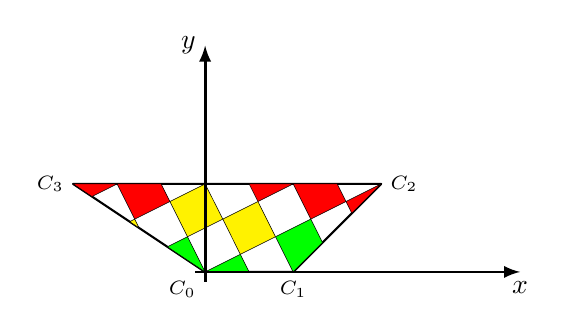
\begin{tikzpicture}[line join=round,line width=0.2pt,>=latex]
\filldraw[fill=none,line width=0.75pt](0,-8)--(1.118,-8)--(2.236,-6.882)--(-1.677,-6.882)--cycle;
\filldraw[fill=red](1.863,-7.255)--(2.236,-6.882)--(1.789,-7.106)--cycle;
\filldraw[fill=red](1.342,-7.329)--(1.789,-7.106)--(1.677,-6.882)--(1.118,-6.882)--cycle;
\filldraw[fill=red](.559,-6.882)--(.671,-7.106)--(1.118,-6.882)--cycle;
\filldraw[fill=red](-1.118,-6.882)--(-.894,-7.329)--(-.447,-7.106)--(-.559,-6.882)--cycle;
\filldraw[fill=red](-1.677,-6.882)--(-1.437,-7.042)--(-1.118,-6.882)--cycle;
\filldraw[fill=yellow](.447,-7.776)--(.894,-7.553)--(.671,-7.106)--(.224,-7.329)--cycle;
\filldraw[fill=yellow](-.447,-7.106)--(-.224,-7.553)--(.224,-7.329)--(0,-6.882)--cycle;
\filldraw[fill=yellow](-.894,-7.329)--(-.839,-7.441)--(-.958,-7.361)--cycle;
\filldraw[fill=green](1.118,-8)--(1.491,-7.627)--(1.342,-7.329)--(.894,-7.553)--cycle;
\filldraw[fill=green](0,-8)--(.559,-8)--(.447,-7.776)--cycle;
\filldraw[fill=green](0,-8)--(-.224,-7.553)--(-.479,-7.681)--cycle;
\draw[->,line width=1pt](0,-8.125)--(0,-5.125);
\draw[->,line width=1pt](-.125,-8)--(4,-8);

    \coordinate [label=below:$x$] (X) at (4,-8);
    \coordinate [label=left:$y$] (Y) at (0,-5.125);
  
    \coordinate [label=225:\scriptsize$C_0$] (p0C) at (0,-8);
    \coordinate [label=270:\scriptsize$C_1$] (p1C) at (1.118,-8);
    \coordinate [label=000:\scriptsize$C_2$] (p2C) at (2.236,-6.882);
    \coordinate [label=180:\scriptsize$C_3$] (p3C) at (-1.677,-6.882);
  \end{tikzpicture}% End sketch output
